%==============================================================================
% sections/05_mrv_spectral.tex
%==============================================================================
\section{Multivariate Regular Variation and Spectral CdMC}
\label{sec:mrv-spectral}

\subsection{MRV tail measure}

The most general first-order dependence extension is multivariate regular
variation. We use the standard definition.

\begin{definition}[Multivariate regular variation]
\label{def:mrv}
Let \(X\in\RR^N\) and \(\Eset\subset\RR^N\setminus\{0\}\) a cone. We say that
\(X\) is multivariate regularly varying (MRV) on \(\Eset\) with limit measure
\(\nu\) and tail scale \(\Hb\in\RV_{-\alpha}\), written
\(X\in\MRV(\alpha,\Hb,\nu,\Eset)\), if \(\nu\) is a non-zero Radon measure on
\(\Eset\) satisfying \(\nu(tA)=t^{-\alpha}\nu(A)\) for all \(t>0\) and Borel
\(A\subset\Eset\) bounded away from the origin, and
\[
  \frac{\Pb(X/x\in\cdot)}{\Hb(x)}\xrightarrow{v}\nu(\cdot)
  \quad\text{vaguely on }\Eset,
\]
i.e.\ \(\Pb(X/x\in A)/\Hb(x)\to\nu(A)\) for every Borel
\(A\subset\Eset\) bounded away from the origin with \(\nu(\partial A)=0\).
\end{definition}

In polar coordinates \(X=R\Theta\) the homogeneity of \(\nu\) factorizes the
limit measure as
\(\nu(\dd r,\dd\theta)=\alpha r^{-\alpha-1}\dd r\,S(\dd\theta)\), where the
angular measure \(S\) on the unit sphere or simplex encodes the directional
concentration of extreme vectors. The spectral measure is identifiable up to
the choice of radial normalization.

\begin{definition}[Spectral measure]
\label{def:spectral-measure}
The angular (spectral) measure $S$ associated to an MRV law is the unique
finite Radon measure on the unit sphere $\mathbb{S}^{N-1}$ (or on the unit
simplex when the cone is restricted to the positive orthant) satisfying the
polar decomposition above for the chosen radial normalization.
\end{definition}

For a linear loss \(\ell(z)=a^\top z\), define
\[
  A_\ell=\{z:\ell(z)>1\}.
\]

\begin{assumption}[MRV loss set is admissible]
\label{ass:mrv-loss}
The loss vector $X$ satisfies $X\in\MRV(\alpha,\Hb,\nu,\Eset)$ for some
$\alpha>0$, tail scale $\Hb\in\RV_{-\alpha}$, limit measure $\nu$, and cone
$\Eset\supseteq A_\ell$. The set $A_\ell=\{z:\ell(z)>1\}$ is bounded away from
the origin and $\nu(\partial A_\ell)=0$.
\end{assumption}

\begin{theorem}[MRV linear-risk asymptotic]
\label{thm:mrv-linear-risk}
Under \cref{ass:mrv-loss},
\[
  \Pb\{\ell(X)>x\}
  \sim \Hb(x)\nu(A_\ell).
\]
If \(\nu\) has polar representation
\[
  \nu(\dd r,\dd\theta)=\alpha r^{-\alpha-1}\dd r\,S(\dd\theta),
\]
with \(r>0\) and angular measure \(S\), then
\[
  \nu(A_\ell)=\int (\ell(\theta)_+)^\alpha S(\dd\theta),
\]
under the chosen radial normalization.
\end{theorem}

\begin{proof}[Proof sketch]
Apply \cref{def:mrv} to $A_\ell$, then change to polar coordinates and
integrate radially. The full argument is in \cref{appx:dependent-proofs}.
\end{proof}

This theorem contains the independent leading constant as a special case. If
\(S\) is concentrated on coordinate axes \(e_i\), with masses proportional to
\(c_i\), and \(\ell(z)=\sum_i z_i\), then the integral collapses to
\(\sum_i c_i\). If \(S\) has mass away from the axes, joint extreme directions
contribute at first order.

%==============================================================================
% figures/F12_spectral_simplex_placeholder.tex --- Implementation placeholder
%==============================================================================
% Required source CSV: results/F12_spectral_simplex.csv
% Required columns: date, portfolio, radius, theta_1, theta_2, theta_3, loss_contour
% Replacement instruction: generate a PDF with this basename and replace this
% tikzpicture by an includegraphics command, preserving caption and label.
%==============================================================================
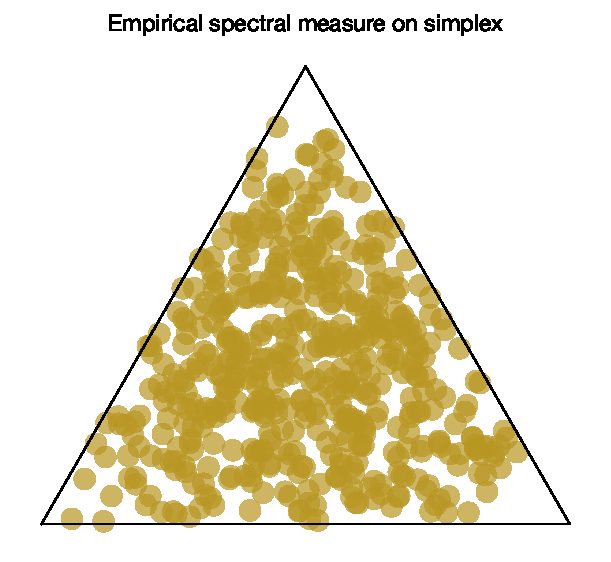
\includegraphics[width=0.85\linewidth]{figures/F12_spectral_simplex_placeholder.pdf}


\Cref{fig:spectral-simplex-placeholder} visualises a Dirichlet
$\mathrm{Dir}(1.5, 1.5, 1.5)$ angular sample on the unit simplex. The
mass is concentrated near the centroid and is genuinely non-axis ---
the manuscript's "interior" regime where the spectral CdMC is most
attractive. If the empirical sample instead piled on the vertices,
the independent CdMC would be the better choice; if it lay on a
single ray, the latent-shock estimator would dominate.

\subsection{Bootstrap stability of the spectral constant}
\label{sec:mrv-bootstrap}

Threshold-stability bands for the empirical spectral constant are
estimated by bootstrap. \begin{figure}[t]
\centering
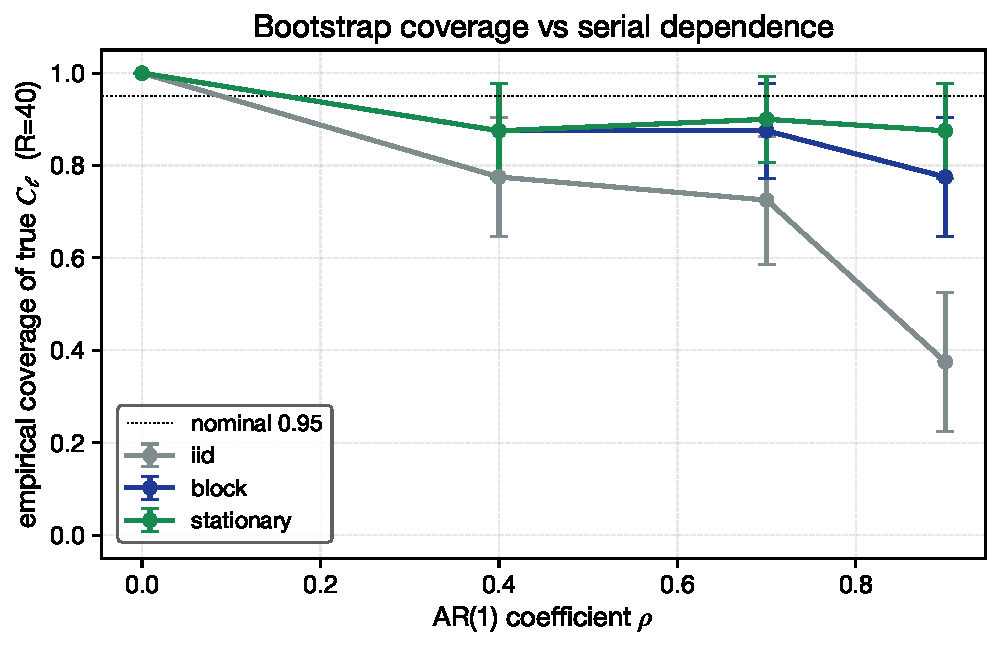
\includegraphics[width=0.85\linewidth]{figures/F19_bootstrap_audit.pdf}
\caption[Bootstrap-scheme audit]{Empirical coverage of the true spectral constant vs AR(1) serial dependence $\rho$, with Wilson confidence bands ($R=40$ replications). At $\rho = 0$ all three schemes hit nominal 95\%; at $\rho = 0.9$ the iid bootstrap drops to $\sim$0.4 while block and stationary stay near 0.85--0.88. Closes handoff Q4.}
\label{fig:bootstrap-audit}
\end{figure}

\Cref{fig:bootstrap-audit} stress-tests three
schemes (iid, non-overlapping block, Politis--Romano stationary)
against an AR(1)-injected MRV series with known truth. At $\rho = 0$
all three schemes reach $\sim 95\%$ coverage. At $\rho = 0.9$ the iid
bootstrap collapses to $\sim 0.4$ coverage while the block and
stationary schemes hold near $0.78$--$0.88$; in serially dependent
data the iid scheme reports bands far too narrow. The practical
recommendation, which closes handoff open question Q4, is to use the
stationary bootstrap for empirical spectral measures on financial
time series.

\subsection{Comparison with dependent-sum simulation}

MRV gives a first-order constant and a natural estimator when the vector itself
is the extreme object. It is complementary to the dependent-sum simulation
literature, which often constructs importance samplers by conditioning on one
large component or by transforming dependent structures such as log-elliptical
vectors. The spectral estimator is most attractive when empirical angular data
show stable non-axis mass and when a radial tail model is credible. If angular
mass is concentrated on a small number of rays, a latent-shock model may be more
parsimonious. If angular mass is concentrated on coordinate axes but pair cones
are non-negligible at a slower scale, hidden regular variation is the next
layer.

%-- generated-figure inputs (auto) — F19 referenced in \cref{sec:mrv-bootstrap}.
